\documentclass[12pt]{ociamthesis}  % default square logo 
%\documentclass[12pt,beltcrest]{ociamthesis} % use old belt crest logo
%\documentclass[12pt,shieldcrest]{ociamthesis} % use older shield crest logo

%load any additional packages
\usepackage{amssymb}
\usepackage{listings}

\usepackage{color}
 
\definecolor{codegreen}{rgb}{0,0.6,0}
\definecolor{codegray}{rgb}{0.5,0.5,0.5}
\definecolor{codepurple}{rgb}{0.58,0,0.82}
\definecolor{backcolour}{rgb}{0.95,0.95,0.92}
 
\lstdefinestyle{mystyle}{
    backgroundcolor=\color{backcolour},   
    commentstyle=\color{codegreen},
    keywordstyle=\color{magenta},
    numberstyle=\tiny\color{codegray},
    stringstyle=\color{codepurple},
    basicstyle=\footnotesize,
    breakatwhitespace=false,         
    breaklines=true,                 
    captionpos=b,                    
    keepspaces=true,                 
    numbers=left,                    
    numbersep=5pt,                  
    showspaces=false,                
    showstringspaces=false,
    showtabs=false,                  
    tabsize=2,
    language=python
}
 
\lstset{style=mystyle}

%input macros (i.e. write your own macros file called mymacros.tex 
%and uncomment the next line)
%\include{mymacros}

\title{Modul Praktikum \\[1ex]     %your thesis title,
        Pemrograman II}   %note \\[1ex] is a line break in the title

\author{Almi Bachri}             %your name
\college{1184043\\[5ex]
Applied Bachelor of Informatics Engineering}  %your college

%\renewcommand{\submittedtext}{change the default text here if needed}
\degree{Politeknik Pos Indonesia}     %the degree
\degreedate{Bandung 2019}         %the degree date

%end the preamble and start the document
\begin{document}

%this baselineskip gives sufficient line spacing for an examiner to easily
%markup the thesis with comments
\baselineskip=18pt plus1pt

%set the number of sectioning levels that get number and appear in the contents
\setcounter{secnumdepth}{3}
\setcounter{tocdepth}{3}


\maketitle                  % create a title page from the preamble info
\begin{dedication}
`Jika Kamu tidak dapat menahan lelahnya belajar, \\
Maka kamu harus sanggup menahan perihnya Kebodohan.'\\ 
~Imam Syafi'i~\\
\end{dedication}        % include a dedication.tex file
\begin{acknowledgements}
Pertama-tama kami panjatkan puji dan syukur kepada Allah SWT yang telah memberikan rahmat dan hidayah-Nya sehingga Modul Praktikum ini dapat diselesaikan.
\end{acknowledgements}   % include an acknowledgements.tex file
\begin{abstract}
	Modul Praktikum ini dibuat dengan tujuan memberikan acuan, bagi mahasiswa dan dosen
	Pengajar Mata Kuliah. Pada intinya buku ini menjelaskan secara lengkap tentang Standar penilian mata kuliah pemrograman II
	di Program Studi D4 Teknik Informatika, dan juga mengatur mekanisme, teknik penulisan, serta
	penilaiannya.Dengan demikian diharapkan semua pihak yang terlibat dalam aktivitas belajar dan mengajar
	berjalan lancar dan sesuai dengan standar.
\end{abstract}          % include the abstract

\begin{romanpages}          % start roman page numbering
\tableofcontents            % generate and include a table of contents
\listoffigures              % generate and include a list of figures
\end{romanpages}            % end roman page numbering

%now include the files of latex for each of the chapters etc
%\chapter{Mengenal Python dan Anaconda}
Tujuan pembelajaran pada pertemuan pertama antara lain:
\begin{enumerate}
\item
Mengerti sejarah python, perkembangan dan penggunaan python di perusahaan
\item
Memahami tahapan instalasi python dan anaconda
\item
Memahami cara penggunaan spyder
\end{enumerate}
Tugas dengan cara dikumpulkan dengan pull request ke github dengan menggunakan format latex pada repo yang dibuat oleh asisten IRC.

\section{Teori}
Praktek teori penunjang yang dikerjakan :
\begin{enumerate}
\item
Buat Resume Sejarah Python, perbedaan python 2 dan 3, dengan bahasa yang mudah dipahami dan dimengerti. Buatan sendiri bebas plagiat(10)
\item
Buat Resume Implementasi dan penggunaan Python di perusahaan dunia, bahasa yang mudah dipahami(10)
\end{enumerate}

\section{Instalasi}
Melakukan instalasi python dan anaconda versi 3 serta uji coba spyder. Dengan menggunakan bahasa yang mudah dimengerti dan bebas plagiat. 
Dan wajib skrinsut dari komputer sendiri.
\begin{enumerate}
\item
Instalasi python 3 (5)
\item
instalasi pip(5)
\item
cara setting environment (5)
\item
mencoba entrepreter/cli melakui terminal atau cmd windows(5)
\item 
Menjalankan dan mengupdate anaconda dan spyder(5)
\item
Cara menjalankan Script hello word di spyder(5)
\item
Cara menjalankan Script otomatis login aplikasi akademik dengan library selenium dan inputan user(5)
\item
Cara pemakaian variable explorer di spyder(5)
\end{enumerate}


\section{Identasi}
Membuat file main.py dan mengisinya dengan script contoh python penggunaan selenium(minimal 20 baris) yang melibatkan inputan user, kemudian mencoba untuk mengatasi error identasi.
\begin{enumerate}
	\item
Penjelasan Identasi (10)
	\item
jenis jenis error identasi yang didapat(10)
\item
cara membaca error(10)
\item 
cara menangani errornya(10)
\end{enumerate}

\section{Presentasi Tugas}
Pada pertemuan ini, diadakan tiga penilaiain yaitu penilaian untuk tugas mingguan dengan nilai maksimal 100. Kemudian dalam satu minggu kedepan maksimal sebelum waktu mata kuliah. Ada presentasi kematerian dengan nilai presentasi yang terpisah masing-masing 100. Dan nilai terpisah untuk tutorial dari jawaban tugas di YouTube.Jadi ada tiga komponen penilaiain pada pertemuan ini yaitu :
\begin{enumerate}
	\item tugas minggu hari ini dan besok (maks 100). pada chapter ini
	\item presentasi csv (maks 100). Mempraktekkan kode python dan menjelaskan cara kerjanya.
	\item pembuatan video tutorial youtube tentang tutorial dari jawaban tugas.(nilai maks 100)
\end{enumerate}
Waktu presentasi pada jam kerja di IRC. Kriteria penilaian presentasi sangat sederhana, presenter akan ditanyai 20(10 pertanyaan program, 10 pertanyaan teori) pertanyaan tentang pemahamannya menggunakan python dan program agan dibuat error hingga presenter bisa menyelesaikan errornya. jika presenter tidak bisa menjawab satu pertanyaan asisten maka nilai nol. Jika semua pertanyaan bisa dijawab maka nilai 100. Presentasi bisa diulang apabila gagal, sampai bisa mendapatkan nilai 100 dalam waktu satu minggu kedepan.
\item\textbf{Jawaban Chapter 1}
\begin{enumerate}
\item Python adalah Bahasa pemrograman kelanjutan dari Bahasa pemrograman ABC python pada  Versi terakhir 1.2. yang dikeluarkan oleh CWI yang dikembangkan oleh Guido van Rossum pada tahun 1990 di CWI.Nama Python diciptakan oleh Guino karena pada saat itu Guino cinta pada acara televisi Monty Python s Flying Circus.
\par
Pada tahun 1995, Guido pindah ke CNRI dan mengembangkan pyhton pada tahun 2000 yaitu versi 1.6. Setelah itu Guido dan para pengembang inti pindah ke BeOpen.com berupa perusahaan komersial dan membentuk beOpen PyhtonLabs yang mengeluarkan Pyhton 2.0 dan beberapa dari anggota tim PyhtonLabs pindah ke DigitalCreations
\par
Sekarang pengembangan pyhton dilakukan oleh programmer yang dikoordinir oleh Guido dan Pyhton Software Foundation. Python Software Foundation adalah organisasi non-profit yang dibentuk untuk memegang hak cipta intelektual. Pada sejak python versi 2.1 mencegah pyhton dimiliki oleh perusahaan komersial.Saat ini pyhton telah mencapai 2.6.1 dan versi 3.0
\par
Adapun perbedaan pada pyhton 2 dan 3 yaitu : Syntax untuk mencetak teks atau yang lainnya, Syntax untuk meminta inputan dan hasil dari operator pembagian.

    \item Banyak penggunaan Bahasa pemrograman pyhton dalam sehari hari contohnya pada penerapan pyhton dalam analisis data, menampilkan timline, data scientist dll. Perusahaan yang telah menggunakan pyhton adalah google,youtube,facebook
    ,Instagram,pinterest,dropbox,quora dll.
\end{enumerate}
\textbf{Instalasi}
\begin{enumerate}
\item Instalasi pyhton 3
\begin{itemize}
    \item jalankan aplikasi untuk menginstal dan centang add python lalu klik install now 1.1
    \begin{figure}
        \centering
        \includegraphics[scale=0.5]{figures/1.PNG}
        \caption{Caption}
        \label{fig:my_label}
    \end{figure}
    \item Lalu tunggu proses installasi 1.2
    \begin{figure}
        \centering
        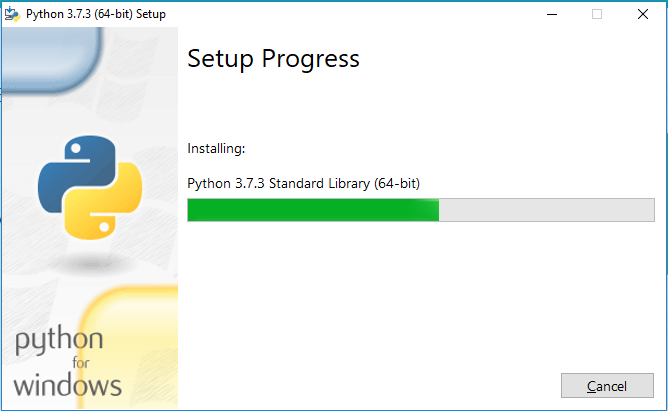
\includegraphics[scale=0.5]{figures/2.PNG}
        \caption{Caption}
        \label{fig:my_label}
    \end{figure}
    \item installasi selesai 1.3
    \begin{figure}
        \centering
        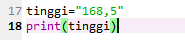
\includegraphics[scale=0.5]{figures/3.PNG}
        \caption{Caption}
        \label{fig:my_label}
    \end{figure}
\end{itemize}
    \item Instalasi PIP
    \begin{itemize}
    \item buka link PIP https://pip.pypa.io/en/stable/installing/ lalu save link yang get-pip.py 1.4
    \begin{figure}
        \centering
        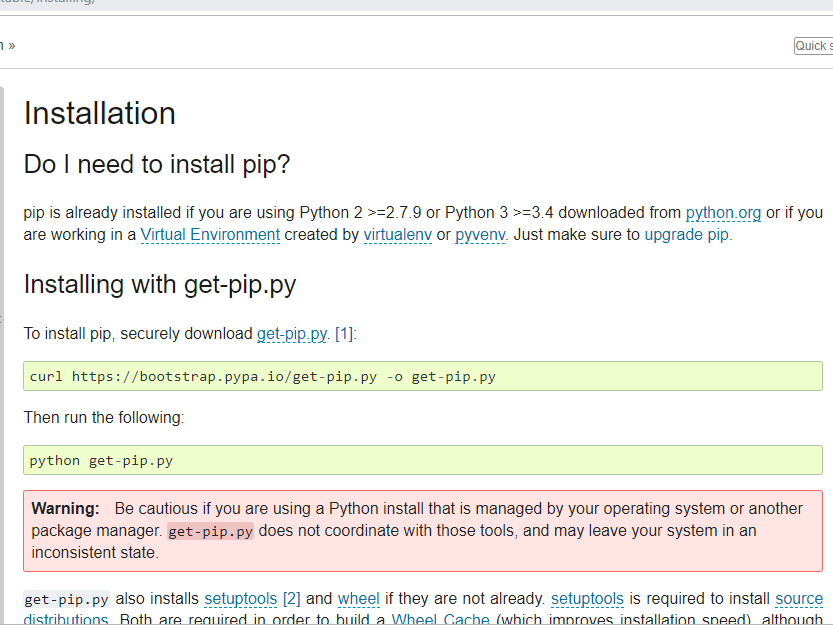
\includegraphics[scale=0.5]{figures/4 (2).PNG}
        \caption{Caption}
        \label{fig:my_label}
    \end{figure}
        \item lalu buka file link yang tadi dengan open with pyhton 1.5 
        \begin{figure}
            \centering
            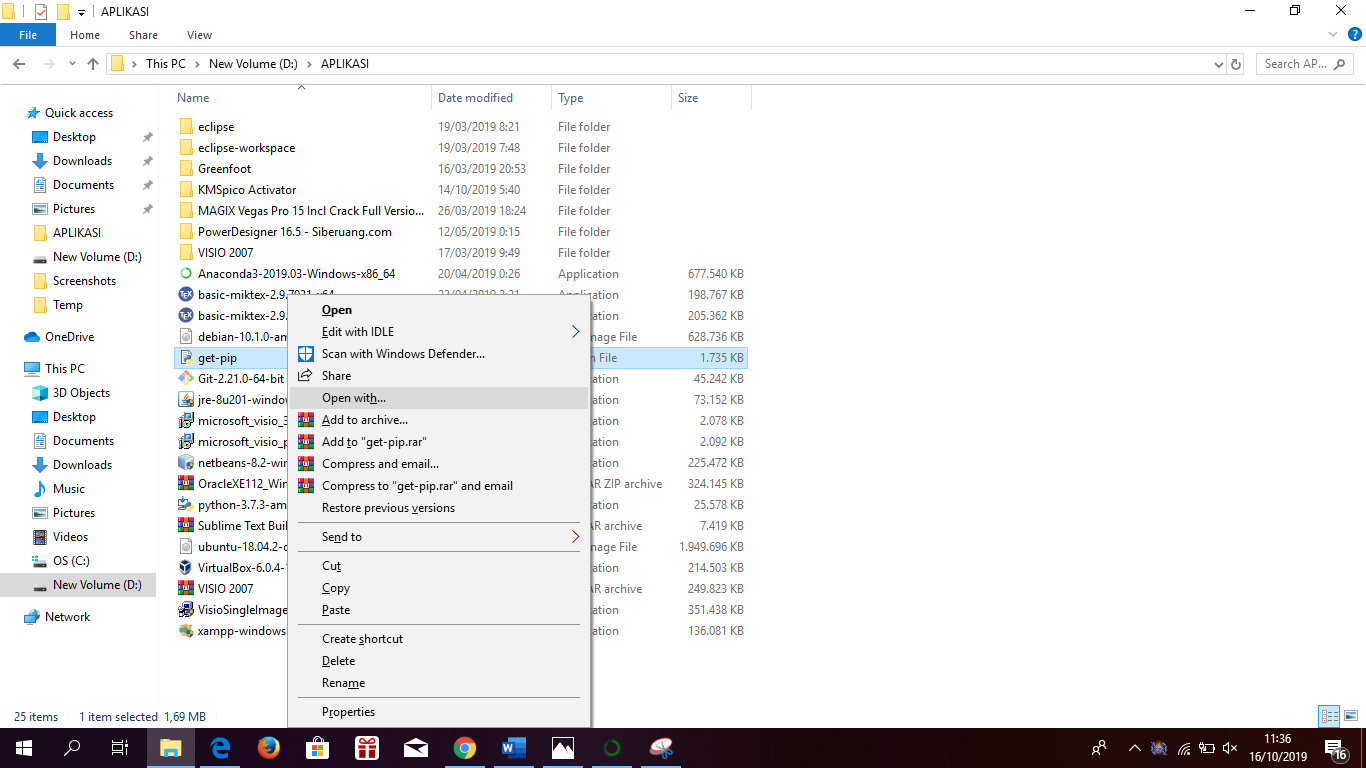
\includegraphics[scale=0.5]{figures/Screenshot (16).png}
            \caption{Caption}
            \label{fig:my_label}
        \end{figure}
        \item setelah dibuka tunggu sampai selesai 1.6
        \begin{figure}
        \centering
        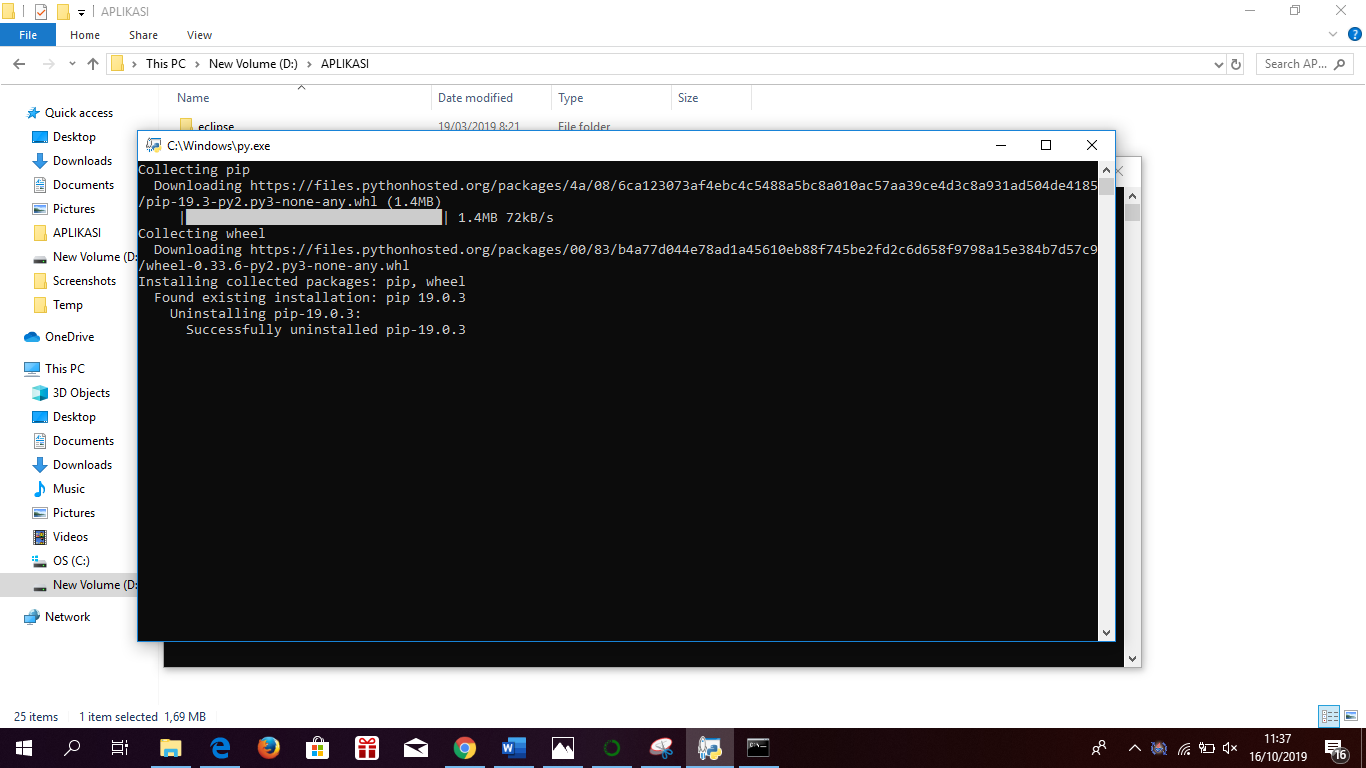
\includegraphics[scale=0.5]{figures/Screenshot (19).png}
            \caption{Caption}
            \label{fig:my_label}
        \end{figure}
    \end{itemize}
    \item cara setting environment
    \begin{itemize}
    \item buka control panel->system & sequrity->system 1.7
    \begin{figure}
    \centering
    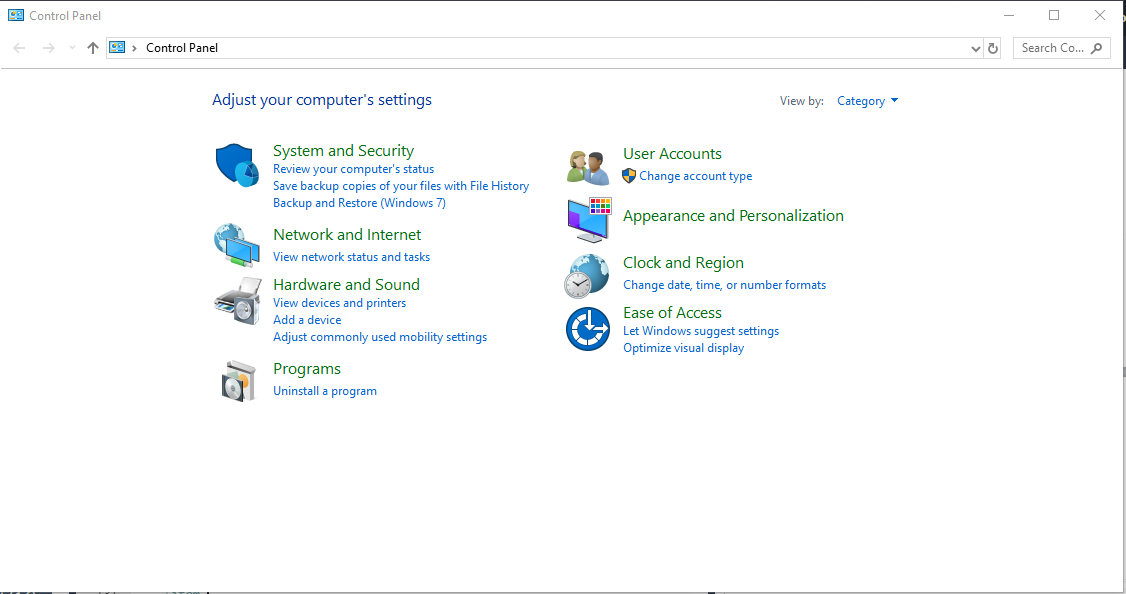
\includegraphics[scale=0.5]{figures/5.PNG}
        \caption{Caption}
        \label{fig:my_label}
    \end{figure}
        \item buka system properties->advance->environments variable 1.8
         \begin{figure}
    \centering
    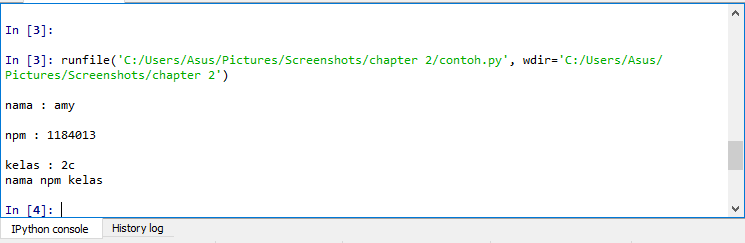
\includegraphics[scale=0.5]{figures/6.PNG}
        \caption{Caption}
        \label{fig:my_label}
    \end{figure}
        \item pada system variable klik dua kali pada path 1.9
         \begin{figure}
    \centering
    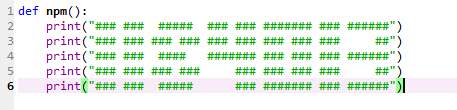
\includegraphics[scale=0.5]{figures/7.PNG}
        \caption{Caption}
        \label{fig:my_label}
    \end{figure}
        \item lalu tambahkan ;c:37 di yang paling atas lalu ok 1.10
         \begin{figure}
    \centering
    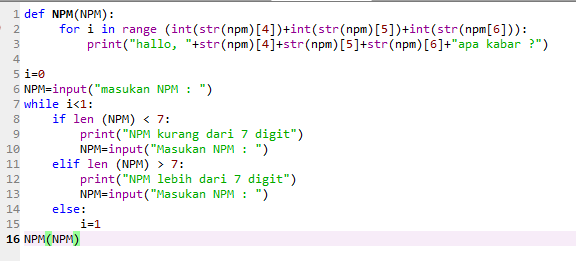
\includegraphics[scale=0.5]{figures/8.PNG}
        \caption{Caption}
        \label{fig:my_label}
    \end{figure}
        \item buka cmd dan tulis pip install request dan enter lalu tunggu 1.11 
         \begin{figure}
    \centering
    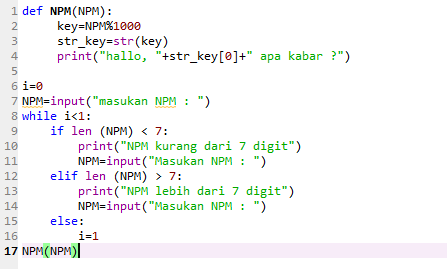
\includegraphics[scale=0.5]{figures/9.PNG}
        \caption{Caption}
        \label{fig:my_label}
    \end{figure}
        \item install berhasil 1.12
         \begin{figure}
    \centering
    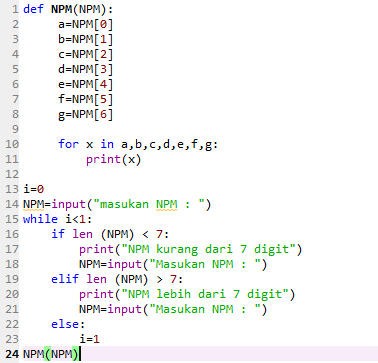
\includegraphics[scale=0.5]{figures/10.PNG}
        \caption{Caption}
        \label{fig:my_label}
    \end{figure}
    \end{itemize}
    \item mencoba entrepreter/cli melakui terminal atau cmd windows 
    \begin{itemize}
    \item buka cmd ->ketik pyhton->lalu ketik yang kita inginkan1.13
    \begin{figure}
    \centering
    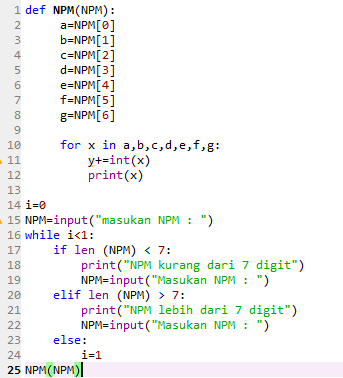
\includegraphics[scale=0.5]{figures/11.PNG}
        \caption{Caption}
        \label{fig:my_label}
    \end{figure}
    \end{itemize}
    \item Menjalankan dan mengupdate anaconda dan spyder
    \begin{itemize}
    \item buka anaconda navigator lalu launch pada spider 1.14
    \begin{figure}
    \centering
    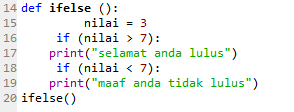
\includegraphics[scale=0.4]{figures/12.PNG}
        \caption{Caption}
        \label{fig:my_label}
    \end{figure}
    \end{itemize}
    \item Cara menjalankan Script hello world di spyder 
    \begin{itemize}
        \item buka aplikasi spider lalu tulis " print ("hello world") " 1.15
        \begin{figure}
    \centering
    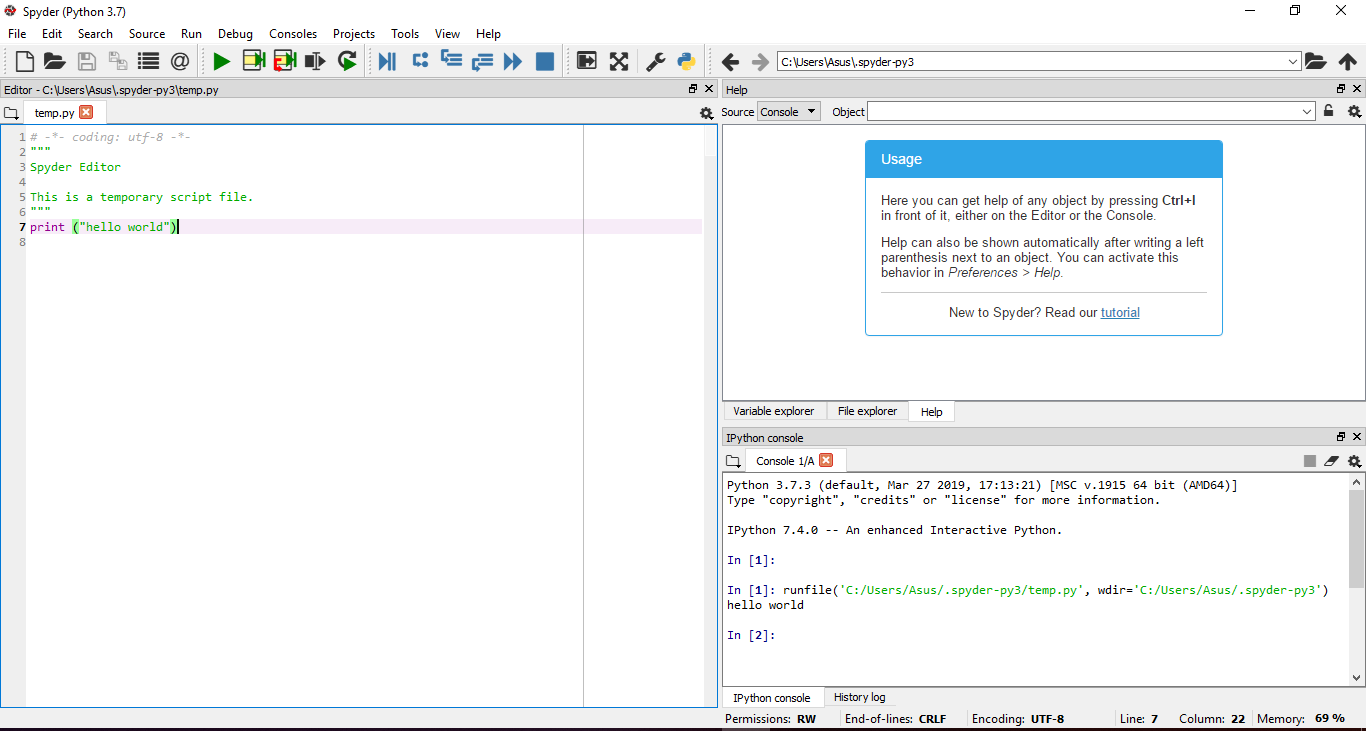
\includegraphics[scale=0.4]{figures/13.PNG}
        \caption{Caption}
        \label{fig:my_label}
    \end{figure}
    \end{itemize}
    \item Cara pemakaian variable explorer di spyder
    \begin{itemize}
    \item buka spyder lalu buat variabelnya seperti di contoh saya lalu di run 1.16
    \begin{figure}
    \centering
    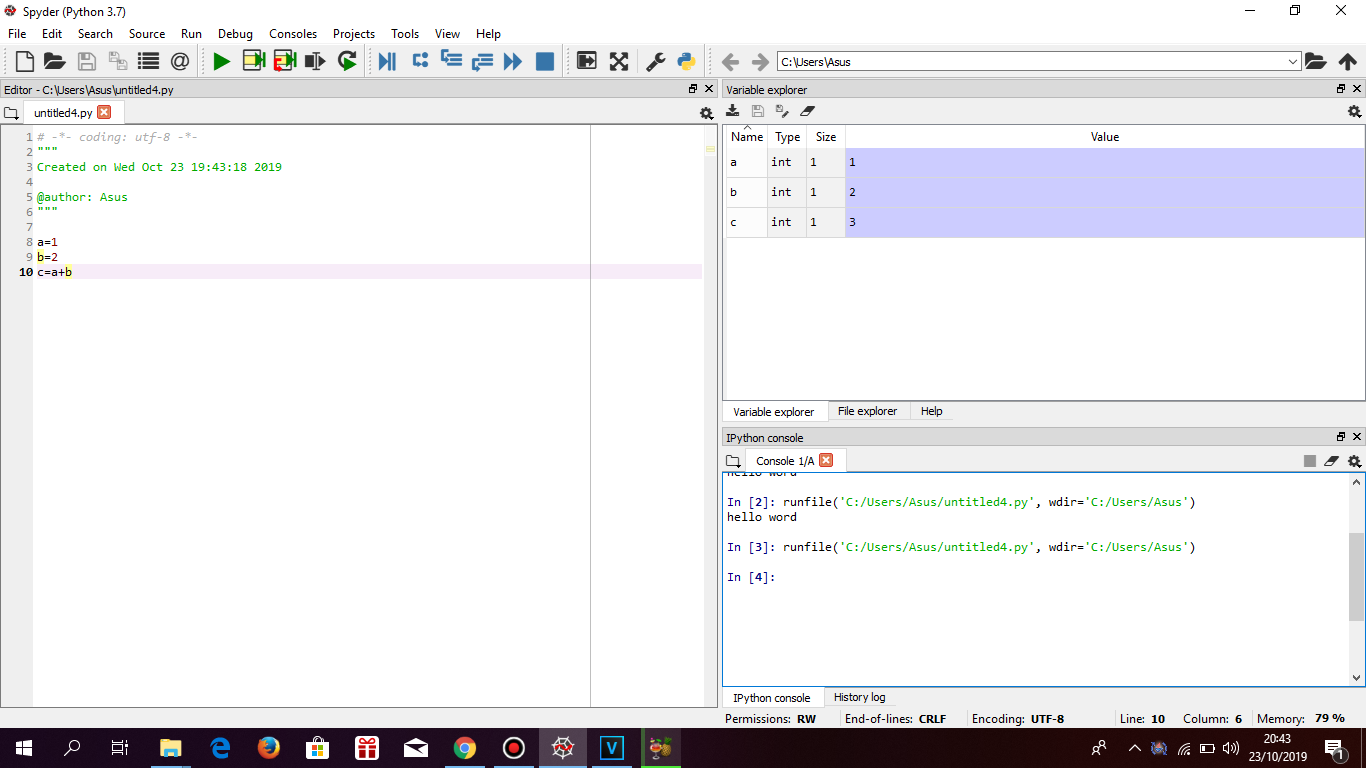
\includegraphics[scale=0.4]{figures/Screenshot (21).png}
        \caption{Caption}
        \label{fig:my_label}
    \end{figure}
    \end{itemize}
\end{enumerate}
%\chapter{Pemrograman Dasar}
Tujuan pembelajaran pada pertemuan kedua antara lain:
\begin{enumerate}
\item
Mengenal Jenis Variabel Python
\item
Input dan output user
\item
Operator Dasar
\item
Perulangan
\item
Kondisi
\item
Mengatasi Error
\item
Try Except
\end{enumerate}
Tugas dengan cara dikumpulkan dengan pull request ke github dengan menggunakan latex pada repo yang dibuat oleh asisten IRC. Kode program dipisah dalam folder src NPM.py yang berisi praktek dari masing-masing tugas file terpisah sesuai nomor yang kemudian dipanggil menggunakan input listing ke dalam file latex penjelasan atau nomor pengerjaan. Masing masing soal bernilai 5 dengan total nilai 100.

\section{Teori}
Praktek teori penunjang yang dikerjakan :
\begin{enumerate}
\item
sebutkan jenis-jenis variabel dan jelaskan cara pemakaian variabel tersebut di kode Python
\item
tuliskan bagaimana kode untuk meminta input dari user dan tuliskan bagaimana melakukan output ke layar
\item
Tuliskan operator dasar aritmatika, tambah, kali, kurang bagi, dan 
bagaimana mengubah string ke integer dan integer ke string
\item
Tuliskan dan jelaskan sintak untuk perulangan, jenis-jenisnya contoh kode dan cara pakainya di python
\item
Tuliskan jelaskan cara pakai sintak untuk memilih kondisi, dan bagiamana contoh sintak kondisi di dalam kondisi.
\item
Tuliskan apa saja jenis error yang sering ditemui di python dalam mengerjakan sintak diatas. 
dan bagaimana cara mengatasinya
\item
Tuliskan dan jelaskan cara memakai Try Except.
\end{enumerate}

\section{Ketrampilan Pemrograman}
Buat program di python dengan ketentuan:
\begin{enumerate}
\item
Buatlah luaran huruf yang dirangkai dari tanda bintang, pagar atau plus dari NPM kita.
Tanda bintang untuk NPM mod 3=0, tanda pagar untuk NPM mod 3 =1, tanda plus untuk NPM mod3=2.
Contoh Output : 
\begin{verbatim}
*****    *** ******     *****    ****
*******  *** ***  **    *** **  *****
***  ******* ******     ***  **** ***
***    ***** ***        ***       ***
***     **** ***        ***       ***
\end{verbatim}
NPM sesuai dengan nomor NPM nya.
\item
Buatlah program hello word dengan input NPM yang disimpan dalam sebuah variabel string bernama \textbf{NPM} dan output sebanyak dua dijit belakang NPM, 
contoh NPM : 113040087 maka akan ada output sebanyak 87 dengan tulisan `Hallo, 113040087 apa kabar?'
\begin{verbatim}
Input : 113040087
Output : 
Halo, 113040087 apa kabar? 
Halo, 113040087 apa kabar?
Halo, 113040087 apa kabar?
Halo, 113040087 apa kabar?
Halo, 113040087 apa kabar?
Halo, 113040087 apa kabar?
Halo, 113040087 apa kabar?
Halo, 113040087 apa kabar?
.....87 kali...
\end{verbatim}
\item
Buatlah program hello word dengan input nama yang disimpan dalam sebuah variabel string bernama \textbf{NPM} dan beri luaran output berupa tiga karakter belakang dari NPM sebanyak penjumlahan tiga dijit tersebut, 
\begin{verbatim}
Input : 113040087
Output : Halo, Nama apa kabar? 
Halo, 087 apa kabar?
Halo, 087 apa kabar?
Halo, 087 apa kabar?
Halo, 087 apa kabar?
Halo, 087 apa kabar?
Halo, 087 apa kabar?
Halo, 087 apa kabar?
........15 kali(0+8+7).........
\end{verbatim}
\item
Buatlah program hello word dengan input nama yang disimpan dalam sebuah variabel string bernama \textbf{NPM} dan beri luaran output berupa digit ketiga dari belakang dari variabel NPM, 
\begin{verbatim}
Input : 113040087
Output :
Halo, 0 apa kabar?
\end{verbatim}
\item
\label{digitvar}
(untuk soal no \ref{digitvar} dan selanjutnya wajib menggunakan perulangan dan kondisi) buat program dengan mengisi variabel alfabet dengan nomor npm satu persatu berurut.
Contoh untuk NPM : 113040087 maka,
\begin{verbatim}
a = 1
b = 1
c = 3
e = 0
f = 4
g = 0
h = 0
i = 8
j = 7
\end{verbatim}
Lakukan print NPM lengkap anda menggunakan variabel diatas :

contoh : 113040087
\item
Dari soal no \ref{digitvar}, Lakukan penjumlahan dari seluruh variabel tersebut,
\item 
Dari soal no \ref{digitvar}, Lakukan perkalian dari seluruh variabel tersebut,
\item
Dari soal no \ref{digitvar}, Lakukan print secara vertikal dari NPM anda menggunakan variabel diatas. Contoh:
\begin{verbatim}
1
1
3
0
4
0
0
8
7
\end{verbatim}
\item
Dari soal no \ref{digitvar}, Lakukan print NPM anda tapi hanya dijit genap saja. Contoh:
\begin{verbatim}
48
\end{verbatim}
\item
Dari soal no \ref{digitvar}, Lakukan print NPM anda tapi hanya dijit ganjil saja. Contoh:
\begin{verbatim}
1137
\end{verbatim}
\item 
Dari soal no \ref{digitvar}, Lakukan print NPM anda tapi hanya dijit yang termasuk bilangan prima saja. Contoh:
\begin{verbatim}
37
\end{verbatim}
\end{enumerate}


\section{Ketrampilan Penanganan Error}
Bagian Penanganan error dari script python.
\begin{enumerate}
\item
Tuliskan peringatan error yang didapat dari mengerjakan praktek kedua ini, dan jelaskan cara penanganan error tersebut.
\item
Membuat file 2err.py dan mengisinya dengan script pengisian variabel sebagai string dan pengisian variabel sebagai interger. 
Kemudian jumlahkan antara variabel integer dan string dan tangkap jenis errornya, gunakan try except untuk menunjukkan error tersebut dengan
bahasa indonesia.
\end{enumerate}


\chapter{Fungsi dan Kelas}
Tujuan pembelajaran pada pertemuan ketiga antara lain:
\begin{enumerate}
\item
Mengenal struktur fungsi di python dalam satu file dan cara pemanggilannya
\item
Mengerti cara membuat library fungsi dan melakukan import dan berbagai jenis import
\item
Mengerti struktur library kelas python dan cara pemakaiannya
\item
Mengatasi Error yang terjadi akibat pemakaian fungsi dan kelas
\item
Try Except
\end{enumerate}
Tugas dengan cara dikumpulkan dengan pull request ke github dengan menggunakan latex pada repo yang dibuat oleh asisten IRC. Kode program dipisah dalam folder src NPM.py yang berisi praktek dari masing-masing tugas file terpisah sesuai nomor yang kemudian dipanggil menggunakan input listing ke dalam file latex penjelasan atau nomor pengerjaan. Masing masing soal bernilai 5 dengan total nilai 100. Gunakan bahasa yang baku dan bebas plagiat dengan dibuktikan hasil scan plagiarisme. Serta hasil scrinsut dari komputer sendiri, dan kode hasil sendiri.

\section{Contoh Program}
\subsection{Fungsi}
Fungsi adalah satu blok program yang terdiri dari nama fungsi, input variabel dan variabel kembalian. Nama fungsi diawali dengan \textit{def} dan setelahnya tanda titik dua. Nama bisa sama dengan isi berbeda jika menggunakan huruf besar dan kecil atau sering disebut dengan \textit{case sensitive}. Input variabel bisa lebih dari satu dengan pemisah tanda koma. variabel kembalian pasti satu, bebas apakan itu jenis \textit{string}, \textit{integer}, \textit{list} atau \textit{dictionary}. Contoh dari fungsi sederhana bisa dilihat pada listing \ref{lst:fungsisederhana}. Dimana hasil akhir variabel c adalah 15.
\begin{lstlisting}[caption=Fungsi Sederhana,label={lst:fungsisederhana}]
def Penambahan(a,b):
	r = a + b
	return r
	
	
a=2
b=13
c = Penambahan(a,b)
\end{lstlisting}
sekarang kita pisah fungsi dengan pemakaian fungsi tersebut dalam file terpisah. Kita buat file bernama \textit{kalkulator.py} yang berisi semua fungsi penambahan, pengurangan, perkalian dan pembagian seperti terlihat pada listing \ref{lst:kalkulatorlib}. Sehingga satu file yang hanya berisi semua fungsi ini kita namakan \textit{paket} atau \textit{library}.
\begin{lstlisting}[caption=Library atau Paket kalkulator,label={lst:kalkulatorlib}]
def Penambahan(a,b):
	r = a + b
	return r
def Pengurangan(a,b):
	r = a - b
	return r
def Perkalian(a,b):
	r = a * b
	return r
def Pembagian(a,b):
	r = a / b
	return r
\end{lstlisting}
	Dan satu file yang memakai fungsi tersebut dengan nama file \textit{main.py}. Karena file kalkulator.py merupakan sebuah library maka kita panggil dulu dengan menggunakan perintah \textit{import}. Harus diingat file \textit{kalkulator.py} harus satu folder dengan \textit{main.py} yang berisi seperti listing\ref{lst:pakaikalkulator}.
\begin{lstlisting}[caption=Cara penggunaan library kalkulator,label={lst:pakaikalkulator}]
import kalkulator

a=100
b=50
hasil1=kalkulator.Penambahan(a,b)
hasil2=kalkulator.Pengurangan(a,b)
hasil3=kalkulator.Perkalian(a,b)
hasil4=kalkulator.Pembagian(a,b)
\end{lstlisting}
Maka kita bisa lihat hasilnya pada variabel hasil1, hasil2, hasil3, hasil4. Pada variabel exporer di spyder.

\subsection{Kelas}
Dasarnya dari kelas adalah pemrograman berbasis objek. Maka kita harus ingat, ada kelas ada objek ada atribut ada method. Fungsi kalkulator kita ubah menjadi kelas Ngitung.py menjadi seperti pada listing \ref{lst:kelasngitung}.
\begin{lstlisting}[caption=Kelas library kalkulator,label={lst:kelasngitung}]
class Ngitung:
  def __init__(self, a, b):
    self.a = a
    self.b = b
  def Penambahan(self):
    r = self.a + self.b
    return r
  def Pengurangan(self):
    r = self.a - self.b
    return r
  def Perkalian(self):
    r = self.a * self.b
    return r
  def Pembagian(self):
    r = self.a / self.b
    return r
\end{lstlisting}
Dana pada file main.py untuk menggunakan kelas maka bedanya adalah penambahan variabel yang menjadi objek instansiasi dari kelas seperti terlihat pada listing \ref{lst:instanngitung}.
\begin{lstlisting}[caption=Cara penggunaan kelas library kalkulator,label={lst:instanngitung}]
import ngitung

a=100
b=50

hitung = ngitung.Ngitung(a,b)

hasil1=hitung.Penambahan()
hasil2=hitung.Pengurangan()
hasil3=hitung.Perkalian()
hasil4=hitung.Pembagian()
\end{lstlisting}



\section{Pemahanan Teori}
Kerjakan soal berikut ini, masing masing bernilai 5. 
Praktek teori penunjang yang dikerjakan :
\begin{enumerate}
\item
Apa itu fungsi, inputan fingsi dan kembalian fungsi dengan contoh kode program lainnya.
\item
Apa itu paket dan cara pemanggilan paket atau library dengan contoh kode program lainnya.
\item
Jelaskan Apa itu kelas, apa itu objek, apa itu atribut, apa itu method dan contoh kode program lainnya masing-masing.
\item
Jelaskan cara pemanggikan library kelas dari instansiasi dan pemakaiannya dengan contoh program lainnya.
\item
Jelaskan dengan contoh pemakaian paket dengan perintah \textit{from kalkulator import Penambahan} disertai dengan contoh kode lainnya.
\item
Jelaskan dengan contoh kodenya, pemakaian paket fungsi apabila file library ada di dalam folder.
\item
Jelaskan dengan contoh kodenya, pemakaian paket kelas apabila file library ada di dalam folder.
\end{enumerate}

\section{Ketrampilan Pemrograman}
Kerjakan soal berikut ini, masing masing bernilai 5. Pada pertemuan sebelumnya tentang pembuatan program di python, sekarang cobalah untuk membuat nya dalam bentuk fungsi dan kelas dengan ketentuan:
\begin{enumerate}
\item
Buatlah fungsi dengan inputan variabel NPM, dan melakukan print luaran huruf yang dirangkai dari tanda bintang, pagar atau plus dari NPM kita.
Tanda bintang untuk NPM mod 3=0, tanda pagar untuk NPM mod 3 =1, tanda plus untuk NPM mod3=2.
Contoh Output : 
\begin{verbatim}
*****    *** ******     *****    ****
*******  *** ***  **    *** **  *****
***  ******* ******     ***  **** ***
***    ***** ***        ***       ***
***     **** ***        ***       ***
\end{verbatim}
NPM sesuai dengan nomor NPM nya.
\item
Buatlah fungsi dengan inputan variabel berupa NPM. kemudian dengan menggunakan perulangan mengeluarkan print output sebanyak dua dijit belakang NPM, 
contoh NPM : 113040087 maka akan ada output sebanyak 87 dengan tulisan `Hallo, 113040087 apa kabar?'
\begin{verbatim}
Output : 
Halo, 113040087 apa kabar? 
Halo, 113040087 apa kabar?
Halo, 113040087 apa kabar?
Halo, 113040087 apa kabar?
Halo, 113040087 apa kabar?
Halo, 113040087 apa kabar?
Halo, 113040087 apa kabar?
Halo, 113040087 apa kabar?
.....87 kali...
\end{verbatim}
\item
Buatlah fungsi dengan dengan input variabel string bernama \textbf{NPM} dan beri luaran output dengan perulangan berupa tiga karakter belakang dari NPM sebanyak penjumlahan tiga dijit tersebut. Penjumlahan dilakukan dengan menggunakan operator aritmatika dan fungsi int() atau str().
\begin{verbatim}
Output : Halo, Nama apa kabar? 
Halo, 087 apa kabar?
Halo, 087 apa kabar?
Halo, 087 apa kabar?
Halo, 087 apa kabar?
Halo, 087 apa kabar?
Halo, 087 apa kabar?
Halo, 087 apa kabar?
........15 kali(0+8+7).........
\end{verbatim}
\item
Buatlah fungsi hello word dengan input variabel string bernama \textbf{NPM} dan beri luaran output berupa digit ketiga dari belakang dari variabel NPM menggunakan akses langsung manipulasi string pada baris ketiga dari variabel NPM.
\begin{verbatim}
Input : 113040087
Output :
Halo, 0 apa kabar?
\end{verbatim}
\item

\label{digitvar2}
(wajib menggunakan perulangan dan atau kondisi) buat fungsi program dengan input variabel NPM dan melakukan print nomor npm satu persatu kebawah.
Contoh untuk NPM : 113040087 maka,
\begin{verbatim}
1
1
3
0
4
0
0
8
7
\end{verbatim}
\item
Buatlah fungsi dengan inputan variabel NPM, didalamnya melakukan penjumlahan dari seluruh dijit NPM tersebut, wajib menggunakan perulangan dan atau kondisi.
\item 
Buatlah fungsi dengan inputan variabel NPM, didalamnya melakukan melakukan perkalian dari seluruh dijit NPM tersebut, wajib menggunakan perulangan dan atau kondisi.
\item
Buatlah fungsi dengan inputan variabel NPM, Lakukan print NPM anda tapi hanya dijit genap saja. wajib menggunakan perulangan dan atau kondisi. Contoh jika NPM :113040087.
\begin{verbatim}
48
\end{verbatim}
\item
Buatlah fungsi dengan inputan variabel NPM, Lakukan print NPM anda tapi hanya dijit ganjil saja. wajib menggunakan perulangan dan atau kondisi. Contoh jika NPM :113040087.
\begin{verbatim}
1137
\end{verbatim}
\item 
Buatlah fungsi dengan inputan variabel NPM, Lakukan print NPM anda tapi hanya dijit yang termasuk bilangan prima saja. wajib menggunakan perulangan dan atau kondisi. Contoh jika NPM :113040087.
\begin{verbatim}
37
\end{verbatim}
\item
Buatlah satu library yang berisi fungsi-fungsi dari nomor diatas dengan nama file 3lib.py dan berikan contoh cara pemanggilannya pada file main.py.
\item
Buatlah satu library class dengan nama file kelas3lib.py yang merupakan modifikasi dari fungsi-fungsi nomor diatas dan berikan contoh cara pemanggilannya  pada file main.py.
\end{enumerate}


\section{Ketrampilan Penanganan Error}
Kerjakan soal berikut ini, masing masing bernilai 5. Bagian Penanganan error dari script python.
\begin{enumerate}
\item
Tuliskan peringatan error yang didapat dari mengerjakan praktek ketiga ini, dan jelaskan cara penanganan error tersebut.
dan Buatlah satu fungsi yang menggunakan gunakan try except untuk menanggulangi error yang kemungkinan akan terjadi.
\end{enumerate}


%\chapter{Pengelolaan File CSV}

Tujuan pembelajaran pada pertemuan keempat antara lain:
\begin{enumerate}
\item
Mengenal file CSV dan fungsinya 
\item
Mengerti cara memakai library CSV
\item
Mengerti cara memakai library pandas
\item
Mengatasi Error yang terjadi akibat pemakaian library csv dan pandas
\item
Try Except
\end{enumerate}
Tugas dengan cara dikumpulkan dengan pull request ke github dengan menggunakan latex pada repo yang dibuat oleh asisten IRC. Kode program dipisah dalam folder src NPM.py yang berisi praktek dari masing-masing tugas file terpisah sesuai nomor yang kemudian dipanggil menggunakan input listing ke dalam file latex penjelasan atau nomor pengerjaan. Masing masing soal bernilai 5 dengan total nilai 100. Gunakan bahasa yang baku dan bebas plagiat dengan dibuktikan hasil scan plagiarisme. Serta hasil scrinsut dari komputer sendiri, dan kode hasil sendiri. Pengerjaan menggunakan latex dan harus menyertakan file pdf hasil compile pdflatex, jika tidak diskon 50\%.


\section{Pemahaman Teori}
Kerjakan soal berikut ini, masing masing bernilai 5. Untuk hari pertama.
Praktek teori penunjang yang dikerjakan dengan deadline besok jam 4 pagi:
\begin{enumerate}
\item
Apa itu fungsi file csv, jelaskan sejarah dan contoh
\par\textbf{Jawaban}
\par CSV (comma separated value) merupakan sebuah file yang berfungsi untuk mempresentasikan sebuah data. format ini termasuk dalam standar file ASCH. file csv juga dapat diimplementasikan dalam beberapa macam perangkat lunak contohnya ms word,oracle,notepad,MySql,sublime dan lain-lain.
\par \textbf{Contoh :}
\par
      \begin{centering}
          \centering
          \includegraphics[scale=1]{figures/chapter 4/1.PNG}
      \end{centering}
\item
Aplikasi-aplikasi apa saja yang bisa menciptakan file csv?
\par \textbf{Jawaban}
\begin{itemize}
    \item Microsoft excel
    \item Notepad
    \item Sublime
    \item Google Sheet
    \item dll
\end{itemize}
\item
Jelaskan bagaimana cara menulis dan membaca file csv di excel atau spreadsheet
\par\textbf{Jawaban}
\begin{itemize}
    \item Buka program microsoft excel atau spreadsheet
    \item Buat data pada baris dan kolom
    \item Lalu save as dan memilih save file dengan .csv
\end{itemize}
\item
Jelaskan sejarah library csv
\par\textbf{Jawaban} 
\par Liblary csv mengimplementasikan kelas yang digunakan untuk membaca dan menulis data dalam format .csv. format ini termasuk dalam standar file ASCH. file csv juga dapat diimplementasikan dalam beberapa macam perangkat lunak contohnya ms word,oracle,notepad,MySql,sublime dan lain-lain.
\item
Jelaskan sejarah library pandas
\par\textbf{Jawaban}
\par Liblaryu pandas adalah pustaka perangkat lunak yang ditulis untuk bahasa pemrograman Python untuk manipulasi dan analisis data.
\item
Jelaskan fungsi-fungsi yang terdapat di library csv
\par\textbf{Jawaban}
\begin{itemize}
    \item Reader
    \par Reader berfungsi untuk membaca file .csv
    \item Write
    \par Write berfungsi untuk membuat file .csv
    \item DictReader
    \par Dictreader berfungsi membaca file .csv dari dictionary
    \item DictWriter   
    \par Dictreader berfungsi untuk membaca file .csv dari dictionary
\end{itemize}
\item
Jelaskan fungsi-fungsi yang terdapat di library pandas
\begin{itemize}
    \item read .csv
    \par fungsi ini digunakan untuk membaca atau membuka file .csv
    \item to.csv
    \par fungsi ini digunakan untuk membuat file .csv
\end{itemize}
\end{enumerate}

\section{Ketrampilan Pemrograman}
Kerjakan soal berikut ini, masing masing bernilai 5 untuk hari kedua, lusa jam 4 pagi. Soalnya adalah:

\begin{enumerate}
\item
Buatlah fungsi (file terpisah/library dengan nama NPM\_csv.py) untuk membuka file csv dengan lib csv mode list
\item
Buatlah fungsi (file terpisah/library dengan nama NPM\_csv.py) untuk membuka file csv dengan lib csv mode dictionary
\item
Buatlah fungsi (file terpisah/library dengan nama NPM\_pandas.py) untuk membuka file csv dengan lib pandas mode list
\item
Buatlah fungsi (file terpisah/library dengan nama NPM\_pandas.py) untuk membuka file csv dengan lib pandas mode dictionary
\item
Buat fungsi baru di NPM\_pandas.py untuk mengubah format tanggal menjadi standar dataframe
\item
Buat fungsi baru di NPM\_pandas.py untuk mengubah index kolom
\item
Buat fungsi baru di NPM\_pandas.py untuk mengubah atribut atau nama kolom
\item
Buat program main.py yang menggunakan library NPM\_csv.py yang membuat dan membaca file csv
\item
Buat program main2.py yang menggunakan library NPM\_pandas.py yang membuat dan membaca file csv
\end{enumerate}




\section{Ketrampilan Penanganan Error}
Kerjakan soal berikut ini, masing masing bernilai 5(hari kedua). Bagian Penanganan error dari script python.
\begin{enumerate}
\item
Tuliskan peringatan error yang didapat dari mengerjakan praktek ketiga ini, dan jelaskan cara penanganan error tersebut.
dan Buatlah satu fungsi yang menggunakan gunakan try except untuk menanggulangi error tersebut.
\begin{itemize}
    \item  berikut errornya yaitu penggunaan variable yang tidak tepat
      \begin{center}
        \centering
        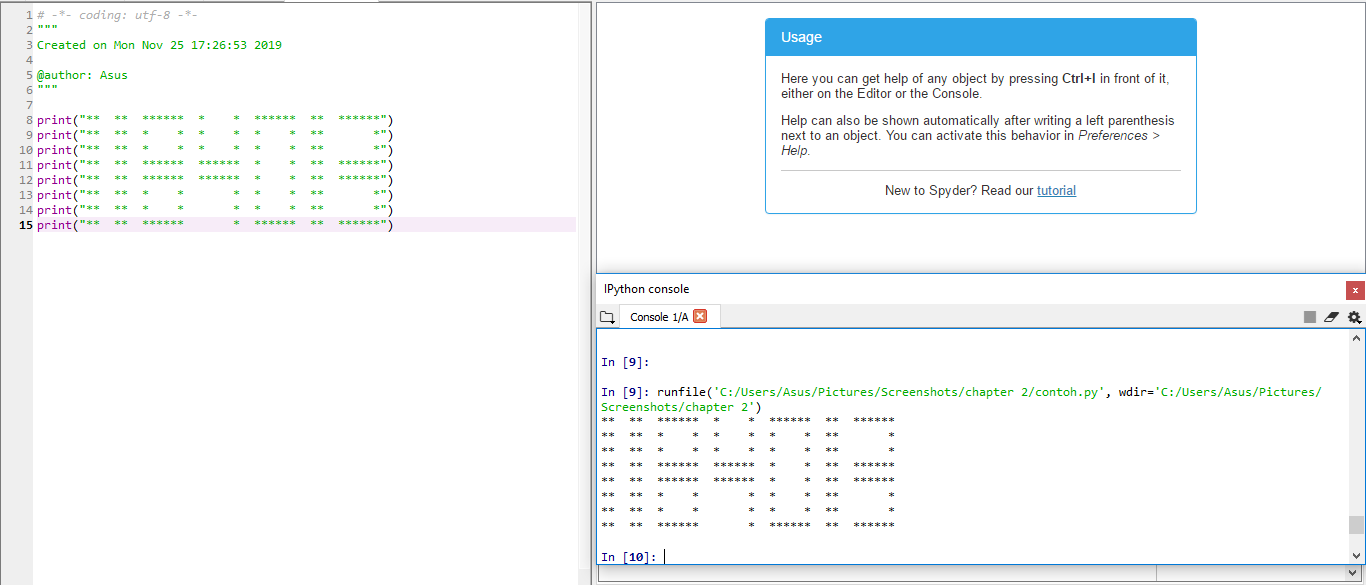
\includegraphics[scale=1]{figures/chapter 3/14.PNG}
    \end{center}
    
        \item  cara penanganannya
      \begin{center}
        \centering
        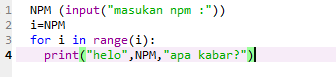
\includegraphics[scale=1]{figures/chapter 3/15.PNG}
    \end{center}
    
    \end{itemize}
\end{enumerate}



\section{Presentasi Tugas}
Pada pertemuan ini, diadakan dua penilaiain yaitu penilaian untuk tugas mingguan seperti sebelumnya dengan nilai maksimal 100. Kemudian dalam satu minggu kedepan maksimal sebelum waktu mata kuliah kecerdasan buatan. Ada presentasi kematerian dengan nilai presentasi yang terpisah masing-masing 100. Jadi ada tiga komponen penilaiain pada pertemuan ini yaitu :
\begin{enumerate}
	\item tugas minggu hari ini dan besok (maks 100). pada chapter ini
	\item presentasi csv (maks 100). Mempraktekkan kode python dan menjelaskan cara kerjanya.
\end{enumerate}
Waktu presentasi pada jam kerja di IRC. Kriteria penilaian presentasi sangat sederhana, presenter akan ditanyai 20(10 pertanyaan program, 10 pertanyaan teori) pertanyaan tentang pemahamannya menggunakan python untuk kecerdasan buatan. jika presenter tidak bisa menjawab satu pertanyaan asisten maka nilai nol. Jika semua pertanyaan bisa dijawab maka nilai 100. Presentasi bisa diulang apabila gagal, sampai bisa mendapatkan nilai 100 dalam waktu satu minggu kedepan.





%\chapter{Komunikasi Perangkat Keras}

Tujuan pembelajaran pada pertemuan kelima antara lain:
\begin{enumerate}
\item
Mengenal komunikasi data serial
\item
Mengerti cara memakai library PySerial
\item
Mengerti cara instalasi driver dan menemukan BaudRate dan Nomor Port
\item
Mengatasi Error yang terjadi akibat pemakaian library csv dan pandas
\item
Try Except
\end{enumerate}
Tugas dengan cara dikumpulkan dengan pull request ke github dengan menggunakan latex pada repo yang dibuat oleh asisten IRC. Kode program dipisah dalam folder src NPM.py yang berisi praktek dari masing-masing tugas file terpisah sesuai nomor yang kemudian dipanggil menggunakan input listing ke dalam file latex penjelasan atau nomor pengerjaan. Masing masing soal bernilai 5 dengan total nilai 100. Gunakan bahasa yang baku dan bebas plagiat dengan dibuktikan hasil scan plagiarisme. Serta hasil scrinsut dari komputer sendiri, dan kode hasil sendiri. Pengerjaan menggunakan latex dan harus menyertakan file pdf hasil compile pdflatex, jika tidak diskon 50\%.


\section{Pemahaman Teori}
Kerjakan soal berikut ini, masing masing bernilai 5. Untuk hari pertama.
Praktek teori penunjang yang dikerjakan dengan deadline rabu jam 4 pagi:
\begin{enumerate}
\item
Apa itu fungsi device manager di windows dan folder /dev di linux
\item
Jelaskan langkah-langkah instalasi driver dari arduino
\item
Jelaskan bagaimana cara membaca baudrate dan port dari komputer yang sudah terinstall driver
\item
Jelaskan sejarah library pyserial
\item
Jelaskan fungsi-fungsi apa saja yang dipakai dari library pyserial
\item
Jelaskan kenapa butuh perulangan dalam tidak butuh perulangan dalam membaca serial
\item
Jelaskan bagaimana cara membuat fungsi yang mengunakan pyserial
\end{enumerate}

\section{Ketrampilan Pemrograman}
Kerjakan soal berikut ini, masing masing bernilai 10 untuk hari kamis jam 4 pagi. Soalnya adalah:

\begin{enumerate}
\item
Buatlah fungsi (file terpisah/library dengan nama NPM\_realtime.py) untuk mendapatkan data langsung dari arduino
\item
Buatlah fungsi (file terpisah/library dengan nama NPM\_save.py) untuk mendapatkan data langsung dari arduino dengan looping
\item
Buatlah fungsi (file terpisah/library dengan nama NPM\_realtime.py) untuk mendapatkan data dari arduino dan langsung ditulis kedalam file csv
\item
Buatlah fungsi (file terpisah/library dengan nama NPM\_csv.py) untuk membaca file csv hasil arduino dan mengembalikan ke fungsi
\end{enumerate}




\section{Ketrampilan Penanganan Error}
Kerjakan soal berikut ini, masing masing bernilai 5(hari kedua). Bagian Penanganan error dari script python.
\begin{enumerate}
\item
Tuliskan peringatan error yang didapat dari mengerjakan praktek ketiga ini, dan jelaskan cara penanganan error tersebut.
dan Buatlah satu fungsi yang menggunakan gunakan try except untuk menanggulangi error tersebut.
\end{enumerate}



\section{Presentasi Tugas}
Pada pertemuan ini, diadakan dua penilaiain yaitu penilaian untuk tugas mingguan seperti sebelumnya dengan nilai maksimal 100. Kemudian dalam satu minggu kedepan maksimal sebelum waktu mata kuliah pemrograman 3. Ada presentasi kematerian dengan nilai presentasi yang terpisah masing-masing 100. Jadi ada tiga komponen penilaiain pada pertemuan ini yaitu :
\begin{enumerate}
	\item tugas minggu hari ini dan besok (maks 100). pada chapter ini
	\item presentasi pyserial (maks 100). Mempraktekkan kode python dan menjelaskan cara kerjanya.
\end{enumerate}
Waktu presentasi pada jam kerja di IRC. Kriteria penilaian presentasi sangat sederhana, presenter akan ditanyai 20(10 pertanyaan program, 10 pertanyaan teori) pertanyaan tentang pemahamannya menggunakan python untuk kecerdasan buatan. jika presenter tidak bisa menjawab satu pertanyaan asisten maka nilai nol. Jika semua pertanyaan bisa dijawab maka nilai 100. Presentasi bisa diulang apabila gagal, sampai bisa mendapatkan nilai 100 dalam waktu satu minggu kedepan.





%\chapter{Matplotlib}

Tujuan pembelajaran pada pertemuan kelima antara lain:
\begin{enumerate}
\item
Mengenal plot di python
\item
Mengerti cara memakai library Matplotlib
\item
Mengerti cara memplot berbagai macam jenis plot
\item
Mengatasi Error yang terjadi akibat pemakaian matplotlib
\item
Try Except
\end{enumerate}
Tugas dengan cara dikumpulkan dengan pull request ke github dengan menggunakan latex pada repo yang dibuat oleh asisten IRC. Kode program dipisah dalam folder src NPM.py yang berisi praktek dari masing-masing tugas file terpisah sesuai nomor yang kemudian dipanggil menggunakan input listing ke dalam file latex penjelasan atau nomor pengerjaan. Masing masing soal bernilai 5 dengan total nilai 100. Gunakan bahasa yang baku dan bebas plagiat dengan dibuktikan hasil scan plagiarisme. Serta hasil scrinsut dari komputer sendiri, dan kode hasil sendiri. Pengerjaan menggunakan latex dan harus menyertakan file pdf hasil compile pdflatex, jika tidak diskon 50\%.


\section{Pemahaman Teori}
Kerjakan soal berikut ini, masing masing bernilai 5. Untuk hari pertama.
Praktek teori penunjang yang dikerjakan dengan deadline hari pertama jam 4 pagi:
\begin{enumerate}
\item
Apa itu fungsi library matplotlib
\item
Jelaskan langkah-langkah membuat sumbu X dan Y di matplotlib
\item
Jelaskan bagaimana perbedaan fungsi dan cara pakai untuk berbagai jenis(bar,histogram,scatter,line dll) jenis plot di matplotlib
\item
Jelaskan bagaimana cara menggunakan legend dan label serta kaitannya dengan fungsi tersebut
\item
Jelaskan apa fungsi dari subplot di matplotlib, dan bagaimana cara kerja dari fungsi subplot, sertakan ilustrasi dan gambar sendiri dan apa parameternya jika ingin menggambar plot dengan 9 subplot di dalamnya
\item
Sebutkan semua parameter color yang bisa digunakan (contoh: m,c,r,k,... dkk)
\item
Jelaskan bagaimana cara kerja dari fungsi hist, sertakan ilustrasi dan gambar sendiri
\item
Jelaskan lebih mendalam tentang parameter dari fungsi pie diantaranya labels, colors, startangle, shadow, explode, autopct
\end{enumerate}

\section{Ketrampilan Pemrograman}
Kerjakan soal berikut ini, masing masing bernilai 10 untuk hari kedua jam 4 pagi. Soalnya adalah:

\begin{enumerate}
\item
Buatlah librari fungsi (file terpisah/library dengan nama NPM\_bar.py) untuk plot dengan jumlah subplot adalah NPM mod 3 + 2
\item
Buatlah librari fungsi (file terpisah/library dengan nama NPM\_scatter.py) untuk plot dengan jumlah subplot NPM mod 3 + 2
\item
Buatlah librari fungsi (file terpisah/library dengan nama NPM\_pie.py) untuk plot dengan jumlah subplot NPM mod 3 + 2
\item
Buatlah librari fungsi (file terpisah/library dengan nama NPM\_plot.py) untuk plot dengan jumlah subplot NPM mod 3 + 2
\end{enumerate}




\section{Ketrampilan Penanganan Error}
Kerjakan soal berikut ini, masing masing bernilai 5(hari kedua). Bagian Penanganan error dari script python.
\begin{enumerate}
\item
Tuliskan peringatan error yang didapat dari mengerjakan praktek ketiga ini, dan jelaskan cara penanganan error tersebut.
dan Buatlah satu fungsi yang menggunakan gunakan try except untuk menanggulangi error tersebut.
\end{enumerate}



\section{Presentasi Tugas}
Pada pertemuan ini, diadakan dua penilaiain yaitu penilaian untuk tugas mingguan seperti sebelumnya dengan nilai maksimal 100. Kemudian dalam satu minggu kedepan maksimal sebelum waktu mata kuliah pemrograman 3. Ada presentasi kematerian dengan nilai presentasi yang terpisah masing-masing 100. Jadi ada tiga komponen penilaiain pada pertemuan ini yaitu :
\begin{enumerate}
	\item tugas minggu hari ini dan besok (maks 100). pada chapter ini
	\item presentasi matplotlib (maks 100). Mempraktekkan kode python dan menjelaskan cara kerjanya.
\end{enumerate}
Waktu presentasi pada jam kerja di IRC. Kriteria penilaian presentasi sangat sederhana, presenter akan ditanyai 20(10 pertanyaan program, 10 pertanyaan teori) pertanyaan tentang pemahamannya menggunakan python untuk kecerdasan buatan. jika presenter tidak bisa menjawab satu pertanyaan asisten maka nilai nol. Jika semua pertanyaan bisa dijawab maka nilai 100. Presentasi bisa diulang apabila gagal, sampai bisa mendapatkan nilai 100 dalam waktu satu minggu kedepan.





%\chapter{Discussion}
Please tell more about conclusion and how to the next work of this study.
%\chapter{Discussion}
Please tell more about conclusion and how to the next work of this study.
%\chapter{Discussion}
Please tell more about conclusion and how to the next work of this study.
%\chapter{Discussion}
Please tell more about conclusion and how to the next work of this study.
%\chapter{Discussion}
Please tell more about conclusion and how to the next work of this study.
%\chapter{Discussion}
Please tell more about conclusion and how to the next work of this study.
%\chapter{Discussion}
Please tell more about conclusion and how to the next work of this study.
%\chapter{Discussion}
Please tell more about conclusion and how to the next work of this study.

%now enable appendix numbering format and include any appendices
\appendix
%\chapter{Form Penilaian Jurnal}

gambar \ref{form1} dan \ref{form2} merupakan contoh bagaimana reviewer menilai jurnal kita. 
\begin{figure}[ht]
      \centerline{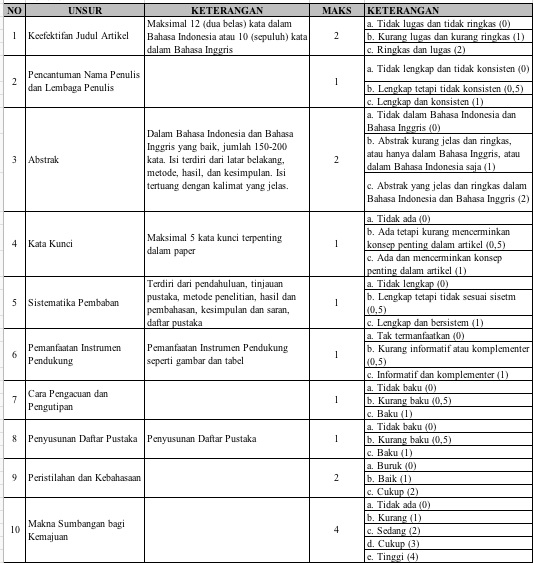
\includegraphics[width=1\textwidth]
      {figures/form1}}
      \caption{Form nilai bagian 1.}
      \label{form1}
      \end{figure}

	\begin{figure}[ht]
	      \centerline{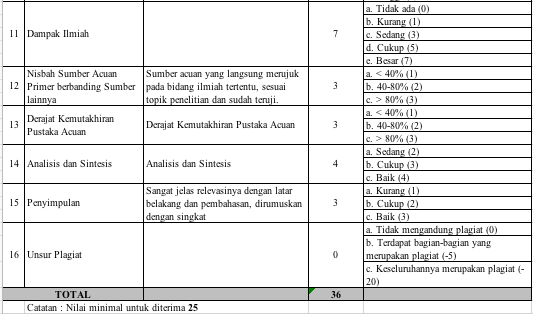
\includegraphics[width=1\textwidth]
	      {figures/form2}}
	      \caption{form nilai bagian 2.}
	      \label{form2}
	      \end{figure}

%\chapter{FAQ}

M : Kalo Intership II atau TA harus buat aplikasi ?
D : Ga harus buat aplikasi tapi harus ngoding

M : Pa saya bingung mau ngapain, saya juga bingung mau presentasi apa?
D : Makanya baca de, buka jurnal topik `ganteng' nah kamu baca dulu sehari 5 kali ya, 4 hari udah 20 tuh. Bingung itu tanda kurang wawasan alias kurang baca.

M : Pa saya sudah cari jurnal terindeks scopus tapi ga nemu.
D : Kamu punya mata de? coba dicolok dulu. Kamu udah lakuin apa aja? tolong di list laporkan ke grup Tingkat Akhir. Tinggal buka google scholar klik dari tahun 2014, cek nama jurnalnya di scimagojr.com beres.

M : Pa saya belum dapat tempat intership, jadi ga tau mau presentasi apa?
D : kamu kok ga nyambung, yang dipresentasikan itu yang kamu baca bukan yang akan kamu lakukan.

M : Pa ini jurnal harus yang terindex scopus ga bisa yang lain ?
D : Index scopus menandakan artikel tersebut dalam standar semantik yang mudah dipahami dan dibaca serta bukan artikel asal jadi. Jika diluar scopus biasanya lebih sukar untuk dibaca dan dipahami karena tidak adanya proses review yang baik dan benar terhadap artikel.

M : Pa saya tidak mengerti
D : Coba lihat standar alasan

M : Pa saya bingung
D : Coba lihat standar alasan

M : Pa saya sibuk
D : Mbahmu....

M : Pa saya ganteng
D : Ndasmu....

M : Pa saya kece
D : wes karepmu lah....


Biasanya anda memiliki alasan tertentu jika menghadapi kendala saat proses bimbingan, disini saya akan melakukan standar alasan agar persepsi yang diterima sama dan tidak salah kaprah. Penggunaan kata alasan tersebut antara lain :

1. Tidak Mengerti : anda boleh menggunakan alasan ini jika anda sudah melakukan tahapan membaca dan meresumekan 15 jurnal. Sudah mencoba dan mempraktekkan teorinya dengan mencari di youtube dan google minimal 6 jam sehari selama 3 hari berturut-turut.

2. Bingung : anda boleh mengatakan alasan bingung setelah maksimal dalam berusaha menyelesaikan tugas bimbingan dari dosen(sudah dilakukan semua). Anda belum bisa mengatakan alasan bingung jika anda masih belum menyelesaikan tugas bimbingan dan poin nomor 1 diatas. Setelah anda menyelesaikan tugas bimbingan secara maksimal dan tahap 1 poin diatas, tapi anda masih tetap bingung maka anda boleh memakai alasan ini.

%next line adds the Bibliography to the contents page
\addcontentsline{toc}{chapter}{Bibliography}
%uncomment next line to change bibliography name to references
%\renewcommand{\bibname}{References}
%\bibliography{references}        %use a bibtex bibliography file refs.bib
\bibliographystyle{plain}  %use the plain bibliography style

\end{document}

